\documentclass[french]{nakrule}

\author{Samuel Riedo \& Pascal Roulin}
\title{Space Invaders}
\subtitle{Projet intégré - Système numérique}

\makeatletter
\let\runauthor\@author
\let\runtitle\@title
\makeatother

\definecolor{mainColor}{RGB}{255,50,50}
\definecolor{blockColor}{RGB}{228,132,132}

\begin{document}


\titleTwo[pictures/title]

%--------------------------------------------------------------------
\chapter{Introduction}
\label{introduction}
%--------------------------------------------------------------------

Space Invaders est un jeu vidéo d'arcade créé par Tomohiro Nishikado, paru pour
la première fois en 1978 au Japon. Il est l'un des tout premier \emph{Shoot 'em
  up}, c'est-à-dire un type de jeux consistant à abatre un grand nombre d'ennemies en
leur tirant dessus. Le principe du jeu consiste en un vasseau spacial attaqué
par des vagues d'aliens qu'il doit détruire sans se faire toucher.

\section{Super Mario Bros}
\label{sec:mario}

Dans un premier temps, nous avions souhaité reproduire \emph{Super Mario Bros}.
La première tentative pour recréer le monde 1-1 du jeu original fut de créer
toute la map en une image de 1600x150, puis de la stocker dans une RAM ou ROM. Ceci
représentait \si{240.000} pixels à stocker. En prenant en compte qu'un pixel
fait exactement un Byte, les RAM et ROM à disposition de la Spartan 6
XC6LX16-CS324 ne pouvait pas stocker toutes ses données.

Afin de contourner ce problème, la carte de base a été diviser en 8 image plus
petite, faisant chacune 200x140 pixels. TODO
néamoins, à la suite de divers problèmes, nous avons finalement prix la décision
de préférer un jeu avec un monde plus petit.

\section{Gameplay}
\label{sec:gameplay}

Space Invaders est un jeu en deux dimension, aussi appelé jeu en 2D ou tout
simplement jeu 2D.


%--------------------------------------------------------------------
\chapter{Architecture}
\label{architecture}


\symmetricalPage

\section{alienRocket}
\label{sec:label}


\begin{center}
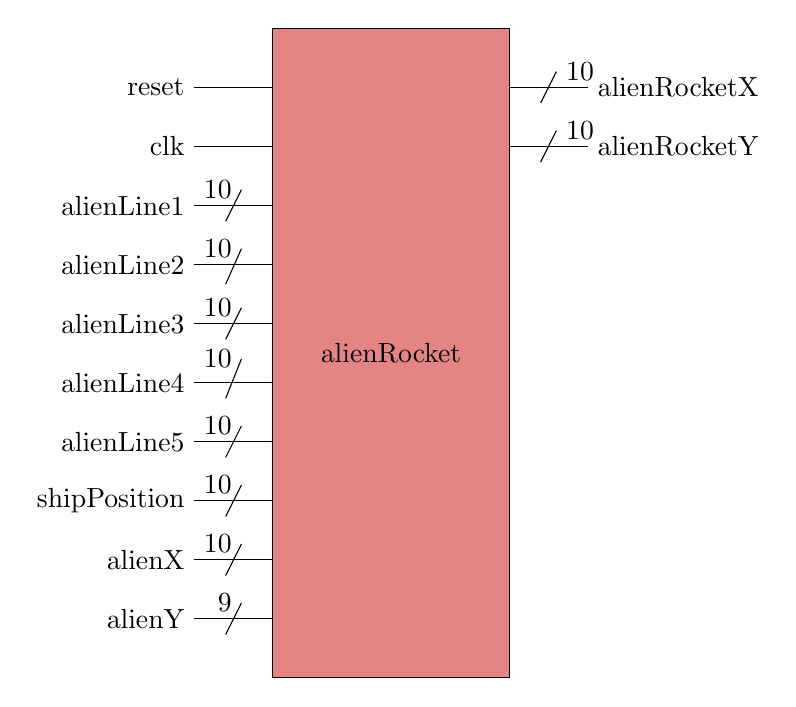
\begin{tikzpicture}
  \draw[fill=blockColor] (0,0) rectangle node{alienRocket}(3,-8.25);
  % Inputs
  \draw (-1,-.75) node[left]{reset}-- (0,-.75);
  \draw (-1,-1.5) node[left]{clk}-- (0,-1.5);
  \draw (-1,-2.25) node[left]{alienLine1}-- (0,-2.25);
  \draw (-.4,-2.05) node[left]{10} -- (-.6, -2.45);
  \draw (-1,-3) node[left]{alienLine2}-- (0,-3);
  \draw (-.4,-2.8) node[left]{10} -- (-.6, -3.25);
  \draw (-1,-3.75) node[left]{alienLine3}-- (0,-3.75);
  \draw (-.4,-3.55) node[left]{10} -- (-.6, -3.95);
  \draw (-1,-4.5) node[left]{alienLine4}-- (0,-4.5);
  \draw (-.4,-4.2) node[left]{10} -- (-.6, -4.7);
  \draw (-1,-5.25) node[left]{alienLine5}-- (0,-5.25);
  \draw (-.4,-5.05) node[left]{10} -- (-.6, -5.45);
  \draw (-1,-6) node[left]{shipPosition}-- (0,-6);
  \draw (-.4,-5.8) node[left]{10} -- (-.6, -6.2);
  \draw (-1,-6.75) node[left]{alienX}-- (0,-6.75);
  \draw (-.4,-6.55) node[left]{10} -- (-.6, -6.95);
  \draw (-1,-7.5) node[left]{alienY}-- (0,-7.5);
  \draw (-.4,-7.3) node[left]{9} -- (-.6, -7.7);
  % Outputs
  \draw (4,-.75) node[right]{alienRocketX}-- (3,-.75);
  \draw (3.6,-.55) node[right]{10} -- (3.4, -.95);
  \draw (4,-1.5) node[right]{alienRocketY}-- (3,-1.5);
  \draw (3.6,-1.3) node[right]{10} -- (3.4, -1.7);
\end{tikzpicture}
\end{center}

\section{DCM}
\label{sec:dcm}

Le composant ressemble à sa:

\begin{center}
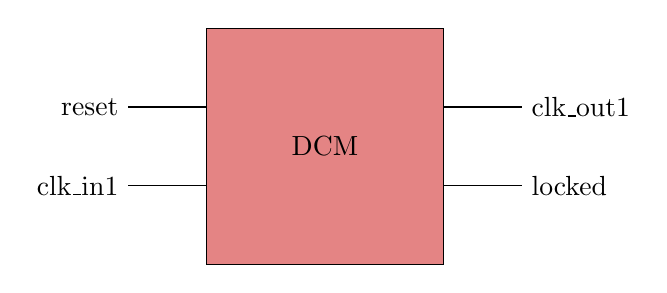
\begin{tikzpicture}
  \draw[fill=blockColor] (0,0) rectangle node{DCM}(3,3);
  \draw (-1,1) node[left]{clk\_in1}-- (0,1);
  \draw (-1,2) node[left]{reset}-- (0,2);
  \draw (4,2) node[right]{clk\_out1}-- (3,2);
  \draw (4,1) node[right]{locked}-- (3,1);
\end{tikzpicture}
\end{center}

\section{Display}
\label{sec:display}


\begin{center}
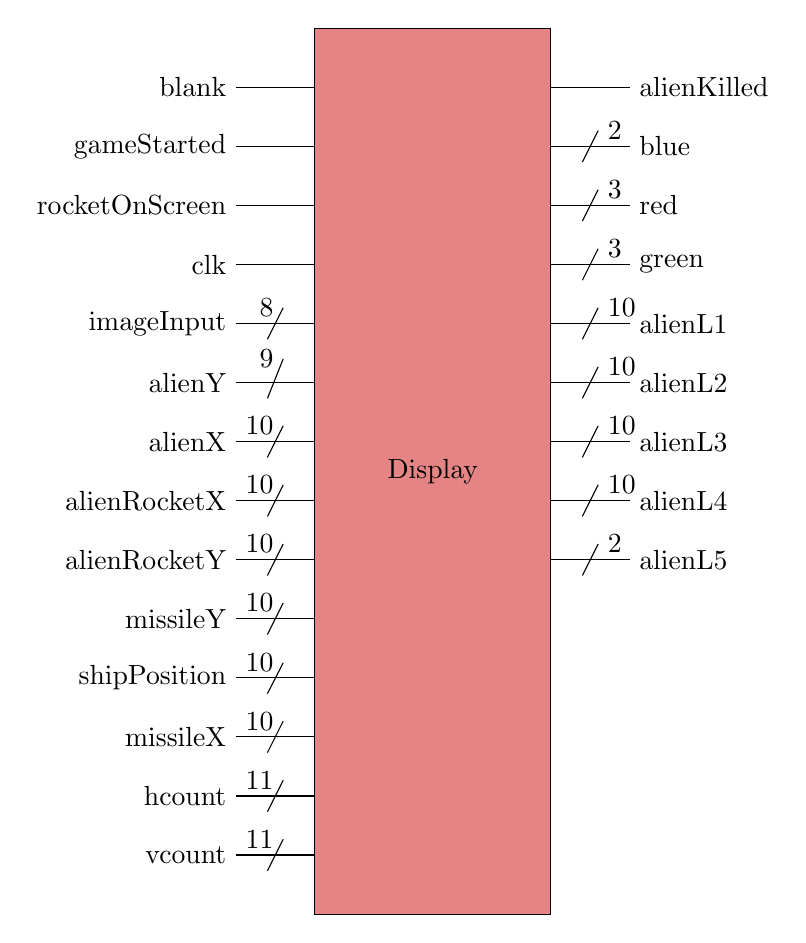
\begin{tikzpicture}
  \draw[fill=blockColor] (0,0) rectangle node{Display}(3,-11.25);
  % Inputs
  \draw (-1,-.75) node[left]{blank}-- (0,-.75);
  \draw (-1,-1.5) node[left]{gameStarted}-- (0,-1.5);
  \draw (-1,-2.25) node[left]{rocketOnScreen}-- (0,-2.25);
  \draw (-1,-3) node[left]{clk}-- (0,-3);
  \draw (-1,-3.75) node[left]{imageInput}-- (0,-3.75);
  \draw (-.4,-3.55) node[left]{8} -- (-.6, -3.95);
  \draw (-1,-4.5) node[left]{alienY}-- (0,-4.5);
  \draw (-.4,-4.2) node[left]{9} -- (-.6, -4.7);
  \draw (-1,-5.25) node[left]{alienX}-- (0,-5.25);
  \draw (-.4,-5.05) node[left]{10} -- (-.6, -5.45);
  \draw (-1,-6) node[left]{alienRocketX}-- (0,-6);
  \draw (-.4,-5.8) node[left]{10} -- (-.6, -6.2);
  \draw (-1,-6.75) node[left]{alienRocketY}-- (0,-6.75);
  \draw (-.4,-6.55) node[left]{10} -- (-.6, -6.95);
  \draw (-1,-7.5) node[left]{missileY}-- (0,-7.5);
  \draw (-.4,-7.3) node[left]{10} -- (-.6, -7.7);
  \draw (-1,-8.25) node[left]{shipPosition}-- (0,-8.25);
  \draw (-.4,-8.06) node[left]{10} -- (-.6, -8.45);
  \draw (-1,-9) node[left]{missileX}-- (0,-9);
  \draw (-.4,-8.8) node[left]{10} -- (-.6, -9.2);
  \draw (-1,-9.75) node[left]{hcount}-- (0,-9.75);
  \draw (-.4,-9.55) node[left]{11} -- (-.6, -9.95);
  \draw (-1,-10.5) node[left]{vcount}-- (0,-10.5);
  \draw (-.4,-10.3) node[left]{11} -- (-.6, -10.7);
  % Outputs
  \draw (4,-.75) node[right]{alienKilled}-- (3,-.75);
  \draw (4,-1.5) node[right]{blue}-- (3,-1.5);
  \draw (3.6,-1.3) node[right]{2} -- (3.4, -1.7);
  \draw (4,-2.25) node[right]{red}-- (3,-2.25);
  \draw (3.6,-2.05) node[right]{3} -- (3.4, -2.45);
  \draw (4,-3) node[right]{green}-- (3,-3);
  \draw (3.6,-2.8) node[right]{3} -- (3.4, -3.2);
  \draw (4,-3.75) node[right]{alienL1}-- (3,-3.75);
  \draw (3.6,-3.55) node[right]{10} -- (3.4, -3.95);
  \draw (4,-4.5) node[right]{alienL2}-- (3,-4.5);
  \draw (3.6,-4.3) node[right]{10} -- (3.4, -4.7);
  \draw (4,-5.25) node[right]{alienL3}-- (3,-5.25);
  \draw (3.6,-5.05) node[right]{10} -- (3.4, -5.45);
  \draw (4,-6) node[right]{alienL4}-- (3,-6);
  \draw (3.6,-5.8) node[right]{10} -- (3.4, -6.2);
  \draw (4,-6.75) node[right]{alienL5}-- (3,-6.75);
  \draw (3.6,-6.55) node[right]{2} -- (3.4, -6.95);
\end{tikzpicture}
\end{center}

\section{Input}
\label{sec:input}


\begin{center}
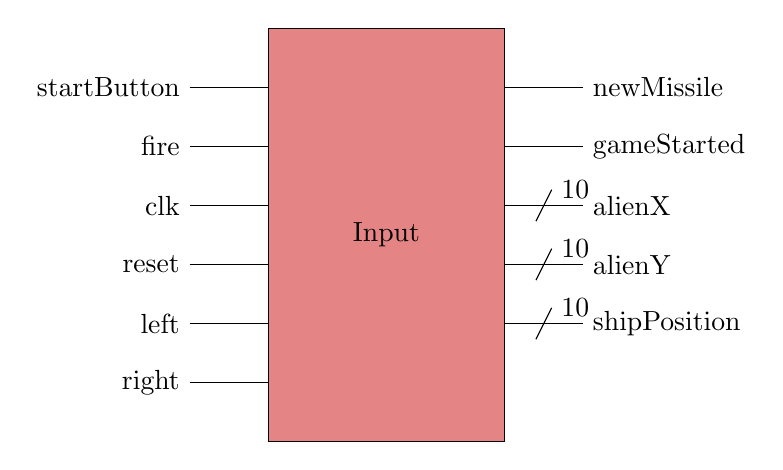
\begin{tikzpicture}
  \draw[fill=blockColor] (0,0) rectangle node{Input}(3,-5.25);
  % Inputs
  \draw (-1,-.75) node[left]{startButton} -- (0,-.75);
  \draw (-1,-1.5) node[left]{fire}-- (0,-1.5);
  \draw (-1,-2.25) node[left]{clk}-- (0,-2.25);
  \draw (-1,-3) node[left]{reset}-- (0,-3);
  \draw (-1,-3.75) node[left]{left}-- (0,-3.75);
  \draw (-1,-4.5) node[left]{right}-- (0,-4.5);
  % Outputs
  \draw (4,-.75) node[right]{newMissile}-- (3,-.75);
  \draw (4,-1.5) node[right]{gameStarted}-- (3,-1.5);
  \draw (4,-2.25) node[right]{alienX}-- (3,-2.25);
  \draw (3.6,-2.05) node[right]{10} -- (3.4, -2.45);
  \draw (4,-3) node[right]{alienY}-- (3,-3);
  \draw (3.6,-2.8) node[right]{10} -- (3.4, -3.2);
  \draw (4,-3.75) node[right]{shipPosition}-- (3,-3.75);
  \draw (3.6,-3.55) node[right]{10} -- (3.4, -3.95);
\end{tikzpicture}
\end{center}


\section{rocketManager}
\label{sec:rocketmanager}

\begin{center}
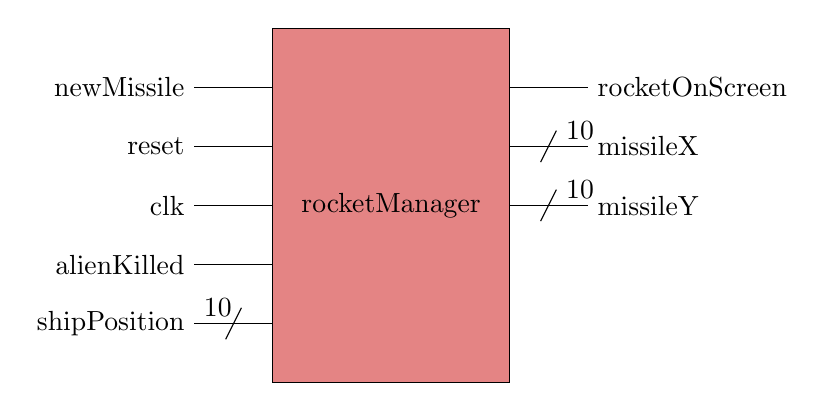
\begin{tikzpicture}
  \draw[fill=blockColor] (0,0) rectangle node{rocketManager}(3,-4.5);
  % Inputs
  \draw (-1,-.75) node[left]{newMissile}-- (0,-.75);
  \draw (-1,-1.5) node[left]{reset}-- (0,-1.5);
  \draw (-1,-2.25) node[left]{clk}-- (0,-2.25);
  \draw (-1,-3) node[left]{alienKilled}-- (0,-3);
  \draw (-1,-3.75) node[left]{shipPosition}-- (0,-3.75);
  \draw (-.4,-3.55) node[left]{10} -- (-.6, -3.95);
  % Outputs
  \draw (4,-.75) node[right]{rocketOnScreen}-- (3,-.75);
  \draw (4,-1.5) node[right]{missileX}-- (3,-1.5);
  \draw (3.6,-1.3) node[right]{10} -- (3.4, -1.7);
  \draw (4,-2.25) node[right]{missileY}-- (3,-2.25);
  \draw (3.6,-2.05) node[right]{10} -- (3.4, -2.45);
\end{tikzpicture}
\end{center}

\section{Top Module}
\label{sec:topmodule}

\begin{center}
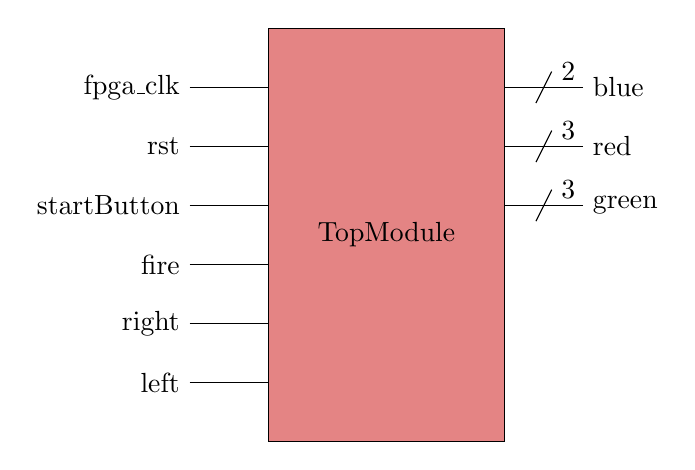
\begin{tikzpicture}
  \draw[fill=blockColor] (0,0) rectangle node{TopModule}(3,-5.25);
  % Inputs
  \draw (-1,-.75) node[left]{fpga\_clk}-- (0,-.75);
  \draw (-1,-1.5) node[left]{rst}-- (0,-1.5);
  \draw (-1,-2.25) node[left]{startButton}-- (0,-2.25);
  \draw (-1,-3) node[left]{fire}-- (0,-3);
  \draw (-1,-3.75) node[left]{right}-- (0,-3.75);
  \draw (-1,-4.5) node[left]{left}-- (0,-4.5);
  % Outputs
  \draw (4,-.75) node[right]{blue}-- (3,-.75);
  \draw (3.6,-.55) node[right]{2} -- (3.4, -.95);
  \draw (4,-1.5) node[right]{red}-- (3,-1.5);
  \draw (3.6,-1.3) node[right]{3} -- (3.4, -1.7);
  \draw (4,-2.25) node[right]{green}-- (3,-2.25);
  \draw (3.6,-2.05) node[right]{3} -- (3.4, -2.45);
\end{tikzpicture}
\end{center}

\section{Package}
\label{sec:package}














\end{document}